% This is text associated with the open textbook "Open Electromagnetics"
% See immediately below for author, date
% This work is licensed under the Creative Commons Attribution-ShareAlike 4.0 International License. (CC BY-SA 4.0) 
% To view a copy of the license, visit http://creativecommons.org/licenses/by-sa/4.0/

%ORB TITLE Resistance
%ORB AUTHOR 0        # S.W. Ellingson, Virginia Tech (ellingson@vt.edu)
%ORB DATE 20180806   # yyyymmdd
%ORB ABSTRACT Resistance at DC

\label{m0071_Resistance_DC} % <-- Must match name of this file and module directory name.  Don't mess with this!
\index{resistance|(}

The concept of resistance is most likely familiar to readers via \emph{Ohm's Law for Devices}; i.e., $V=IR$ where $V$ is the potential difference associated with a current $I$.
This is correct, but it is not the whole story. 
Let's begin with a statement of intent:
%
%ORB HIGHLIGHT
\begin{mdframed}[backgroundcolor=yellow!20,nobreak=true] 
Resistance 
\index{resistance!definition}
$R$ ($\Omega$) is a characterization of the conductivity of a \emph{device} (as opposed to a \emph{material}) in terms of Ohms Law for Devices; i.e., $V=IR$.
\end{mdframed}
%
Resistance is a property of devices such as resistors, which are intended to provide resistance, as well as being a property of most practical electronic devices, whether it is desired or not.  

Resistance is a manifestation of the conductivity of the materials comprising the device, which subsequently leads to the ``$V=IR$'' relationship.  This brings us to a very important point and a common source of confusion.
\emph{Resistance is not necessarily the real part of impedance.}
\index{impedance!of resistance}
Let's take a moment to elaborate.
Impedance ($Z$) is defined as the ratio of voltage to current; i.e., $V/I$; or equivalently in the phasor domain as $\widetilde{V}/\widetilde{I}$.
Most devices -- not just devices exhibiting resistance -- can be characterized in terms of this ratio.
Consider for example the input impedance of a terminated transmission line (Section~\ref{m0087_Input_Impedance_of_a_Terminated_Lossless_Transmission_Line}).  This impedance may have a non-zero real-valued component even when the transmission line and the terminating load are comprised of perfect conductors.
Summarizing:
%ORB HIGHLIGHT
\begin{mdframed}[backgroundcolor=yellow!20,nobreak=true] 
Resistance results in a real-valued impedance. However, not all devices exhibiting a real-valued impedance exhibit resistance.  Furthermore, the real component of a complex-valued impedance does not necessarily represent resistance. 
\end{mdframed}
%
Restating the main point in yet other words: \emph{Resistance pertains to limited conductivity, not simply to voltage-current ratio.}

Also important to realize is that 
whereas conductivity 
\index{conductivity}
$\sigma$ (units of S/m) is a property of materials,
resistance depends on \emph{both} conductivity and the geometry of the device. 
In this section, we address the question of how the resistance of a device can be is determined.
The following example serves this purpose.

\index{resistance!of wire (DC)|(}
\index{wire!DC resistance of|(}

Figure~\ref{m0071_fMatEx1} shows a straight wire 
of length $l$ centered on the $z$ axis, forming a cylinder of material having conductivity $\sigma$ and cross-sectional radius $a$.  
The ends of the cylinder are covered by perfectly-conducting plates to which the terminals are attached.
A battery is connected to the terminals, resulting in a uniform internal electric field ${\bf E}$ between the plates.  
%
\begin{figure}
\begin{center}
\pdftooltip{{  % note double braces
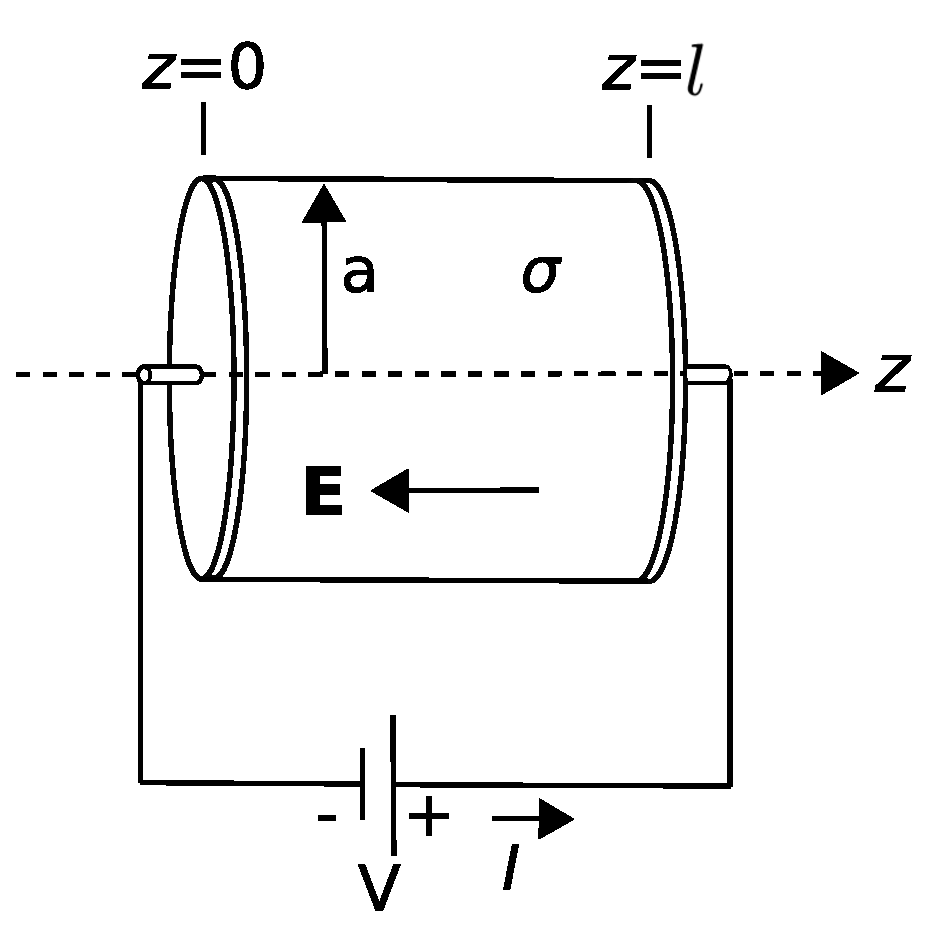
\includegraphics[width=2in]{modules/m0071_fMatEx1.eps}
% https://commons.wikimedia.org/wiki/File:M0071_fMatEx1.svg
}}{A three-dimensional wire with radius a, length l, and conductivity sigma lies on its side centered on the z-axis. On both ends of the wire are two thin plates, with terminals on each side. The left plate is labeled z = 0, and the right plate is labeled z = l. The wire is connected to a battery, with the positive side connected to the right side of the wire with current flowing counterclockwise. The internal electric field in the wire is represented by a vector pointed to the left, labeled E.}
\end{center} 
\centerline{\scriptsize 
\copyright~\hyperref[m0071_fMatEx1_Credit]{K.\ Kikkeri} 
\href{https://creativecommons.org/licenses/by-sa/4.0/}{CC BY~SA 4.0} 
} 
\caption{
\label{m0071_fMatEx1}
Analysis of the resistance of straight wire of circular cross-section. 
}
\end{figure}

To calculate $R$ for this device, let us first calculate $V$, then $I$, and finally $R=V/I$.  
First, we compute the potential difference using the following result from Section~\ref{m0061_Force_Energy_and_Potential_Difference}:
%
\begin{equation}
V = -\int_{\mathcal C}{\bf E}\cdot d{\bf l}
\end{equation}
%
Here we can view $V$ as a ``given'' (being the voltage of the battery), but wish to evaluate the right hand side so as to learn something about the effect of the conductivity and geometry of the wire.
The appropriate choice of ${\mathcal C}$ begins at $z=0$ and ends at $z=l$, following the axis of the cylinder.
(Remember: ${\mathcal C}$ defines the reference direction for increasing potential, so the resulting potential difference will be the node voltage at the end point minus the node voltage at the start point.)
Thus, $d{\bf l} = \hat{\bf z}dz$ and we have
%
\begin{flalign}
V &= -\int_{z=0}^{l} {\bf E} \cdot \left(\hat{\bf z}dz\right) \nonumber
\end{flalign} 
%
We do not yet know ${\bf E}$; however, we know it is constant throughout the device and points in the $-\hat{\bf z}$ direction since this is the direction of current flow and Ohm's Law for Electromagnetics (Section~\ref{m0010_Conductivity}) requires the electric field to point in the same direction.
Thus, we may write ${\bf E}=-\hat{\bf z}E_z$ where $E_z$ is a constant.
We now find:
%
\begin{flalign}
V &= -\int_{z=0}^{l} \left(-\hat{\bf z}E_z\right) \cdot \left(\hat{\bf z}dz\right) \nonumber \\
  &= +E_z \int_{z=0}^{l} dz \nonumber \\
  &= +E_z l \nonumber
\end{flalign} 

The current $I$ is given by (Section~\ref{m0101_Current_Distributions})
%
\begin{flalign}
I &= \int_{\mathcal{S}} {\bf J} \cdot d{\bf s} \nonumber
\end{flalign}
%
We choose the surface $\mathcal{S}$ to be the cross-section perpendicular to the axis of the wire. 
Also, we choose $d{\bf s}$ to point such that $I$ is positive with respect to the sign convention shown in Figure~\ref{m0071_fMatEx1}.
With these choices, we have
%
\begin{flalign}
I &= \int_{\rho=0}^a\int_{\phi=0}^{2\pi} {\bf J} \cdot \left( -\hat{\bf z}~\rho~d\rho~d\phi \right) \nonumber
\end{flalign}
%
From Ohm's Law for Electromagnetics, we have
%
\begin{equation}
{\bf J} = \sigma{\bf E} = -\hat{\bf z} \sigma E_z
\end{equation}
%
So now
%
\begin{flalign}
I &= \int_{\rho=0}^a\int_{\phi=0}^{2\pi} \left( -\hat{\bf z} \sigma E_z  \right) \cdot \left(-\hat{\bf z}\rho~d\rho~d\phi \right) \nonumber \\
  &= \sigma E_z \int_{\rho=0}^a\int_{\phi=0}^{2\pi} \rho~d\rho~d\phi \nonumber \\
  &= \sigma E_z \left( \pi a^2 \right) \nonumber
\end{flalign}     
%
Finally:
%
\begin{equation}
R = \frac{V}{I} 
  = \frac{E_z l}{\sigma E_z \left( \pi a^2 \right)} 
  = \frac{l}{\sigma \left( \pi a^2 \right)} \nonumber 
\end{equation}
%
This is a good-enough answer for the problem posed, but it is easily generalized a bit further.  Noting that $\pi a^2$ in the denominator is the cross-sectional area $A$ of the wire, so we find:
%
\begin{equation}
\boxed{
R = \frac{l}{\sigma A}
}
\label{m0071_eRwireDC}
\end{equation}
%
i.e., the resistance of a wire having cross-sectional area $A$ -- regardless of the shape of the cross-section, is given by the above equation.
%
%ORB HIGHLIGHT
\begin{mdframed}[backgroundcolor=yellow!20,nobreak=true] 
The resistance of a right cylinder of material, given by Equation~\ref{m0071_eRwireDC}, is proportional to length and inversely proportional to cross-sectional area and conductivity.
\end{mdframed}

It is important to remember that Equation~\ref{m0071_eRwireDC} presumes that the volume current density ${\bf J}$ is uniform over the cross-section of the wire.  
This is an excellent approximation for thin wires at ``low'' frequencies including, of course, DC.
At higher frequencies it may not be a good assumption that ${\bf J}$ is uniformly-distributed over the cross-section of the wire, and at sufficiently high frequencies one finds instead that the current is effectively limited to the exterior surface of the wire.  
In the ``high frequency'' case, $A$ in Equation~\ref{m0071_eRwireDC} is reduced from the physical area to a smaller value corresponding to the reduced area through which most of the current flows.
Therefore, $R$ increases with increasing frequency.  
To quantify the high frequency behavior of $R$ (including determination of what constitutes ``high frequency'' in this context) one requires concepts beyond the theory of electrostatics, so this is addressed elsewhere.

%----------------------------------------------------------

%ORB EXAMPLE
~\\ \begin{example} 
\begin{mdframed}[backgroundcolor=brown!20,linecolor=brown!20]\raggedright
Resistance of 22~AWG hookup wire.
\\~\\
A common type of wire found in DC applications is 22AWG (``American Wire Gauge''; see ``Additional Resources'' at the end of this section) copper solid-conductor hookup wire.
This type of wire has circular cross-section with diameter 0.644~mm.
What is the resistance of 3~m of this wire? 
Assume copper conductivity of $58$~MS/m.

{\bf Solution.} 
From the problem statement,
the diameter $2a=0.644$~mm,
$\sigma=58\times 10^6$~S/m, and 
$l=3$~m.
The cross-sectional area is $A=\pi a^2 \cong 3.26\times10^{-7}$~m$^2$.
Using Equation~\ref{m0071_eRwireDC} we obtain $R=159$~m$\Omega$.
\end{mdframed}\end{example}

\index{resistance!of wire (DC)|)}
\index{wire!DC resistance of|)}

%-------------------------------------------------------------------------

%ORB EXAMPLE
~\\ \begin{example} 
\begin{mdframed}[backgroundcolor=brown!20,linecolor=brown!20]\raggedright
Resistance of steel 
\index{steel}
pipe.
\index{pipe}
\\~\\
A pipe is 3~m long and has inner and outer radii of 5~mm and 7~mm respectively.
It is made from steel having conductivity 4~MS/m. 
What is the DC resistance of this pipe? 

{\bf Solution.} 
We can use Equation~\ref{m0071_eRwireDC} if we can determine the cross-sectional area $A$ through which the current flows.
This area is simply the area defined by the outer radius, $\pi b^2$, minus the area defined by the inner radius $\pi a^2$.
Thus, $A = \pi b^2 - \pi a^2 \cong 7.54 \times 10^{-5}$~m$^2$.
From the problem statement, we also determine that
$\sigma=4\times 10^6$~S/m and 
$l=3$~m.
Using Equation~\ref{m0071_eRwireDC} we obtain $R \cong 9.95$~m$\Omega$.
\end{mdframed}\end{example}

%-------------------------------------------------------------------------

{\bf Additional Reading:}
\begin{itemize}
\item ``\href{https://en.wikipedia.org/wiki/Resistor}{Resistor}'' on Wikipedia.
\item ``\href{https://en.wikipedia.org/wiki/Ohm's_law}{Ohm's Law}'' on Wikipedia.
\item ``\href{https://en.wikipedia.org/wiki/American_wire_gauge}{American wire gauge}'' on Wikipedia.
\end{itemize}

\index{resistance|)}

